\documentclass[17pt,a0paper]{tikzposter}

% Suppress some useless warnings
\usepackage{silence}
\WarningFilter{remreset}{The remreset package}
\WarningFilter{latex}{Font shape declaration has incorrect series value `mc'.}

% \usetheme{Default}
% \usetheme{Rays}
\usetheme{Basic}
% \usetheme{Simple}
% \usetheme{Envelope}
% \usetheme{Wave}
% \usetheme{Board}
% \usetheme{Autumn}
% \usetheme{Desert}

\usepackage[UKenglish]{babel}
\usepackage[style=alphabetic,maxbibnames=99]{biblatex}
\usepackage{amsmath}
\newcommand{\defeq}{\vcentcolon=}
\usepackage{mathtools}
\usepackage{amsthm}
\usepackage{csquotes}
\usepackage[inline]{enumitem}
\usepackage[capitalize,noabbrev]{cleveref}
\usepackage[final]{microtype}

% Fix me notes
\usepackage[draft]{fixme}
\usepackage{svg}
\fxusetheme{color}

\usepackage[charter]{mathdesign}
\usepackage[T1]{fontenc}

\title{Stochastic Gradient Hamiltonian Monte Carlo}
\author{Sam Adam-Day, Alexander Goodall, Theo Lewy and Fanqi Xu}
\institute{University of Oxford}


% Bibliography
\addbibresource{../references.bib}

\begin{document}

	\maketitle
	
		\begin{columns}

	%%% First column %%%%%%%%%%%%%%%%%%%%%%%%%%%%%%%%%%%%%%%%%%%%%%%%%%%%%
		\column{0.4}
		
	
	%%% Second column %%%%%%%%%%%%%%%%%%%%%%%%%%%%%%%%%%%%%%%%%%%%%%%%%%%%%
	   \column{0.6}
		

    	\end{columns}

	\begin{columns}

		%%% First column %%%%%%%%%%%%%%%%%%%%%%%%%%%%%%%%%%%%%%%%%%%%%%%%%%%%%
		\column{0.5}
		\block{Stochastic Gradient Hamiltonian Monte Carlo}{
		Hamiltonian Monte Carlo (HMC) provides a way to sample from a posterior distribution using all data available to it. To do this it must produce the potential function $U(\theta) \propto \log p(\theta | \mathcal{D})$, as well as its gradient. Using all of the data to find $U(\theta)$ is computationally expensive for large datasets, rendering HMC useless. This motivated the production of the Stochastic Gradient Hamiltonian Monte Carlo algorithm (SGHMC), which is introduced in \cite{sghmc}. It uses batch data to produce noisy estimates of the potential function, which gives SGHMC dramatic speed-up when compared to HMC. In this paper, Chen et al introduce a Naive SGHMC algorithm, as well as SGHMC itself. They demonstrate links between SGHMC and both Stochastic Gradient Descent with momentum, and Stochastic Gradient Langevin Dynamics. They then run experiments using SGHMC. We reproduced SGHMC, and replicated a number of Chen et al's experiments. The repository for our code is found at https://github.com/sacktock/SGHMC.
	
		
	}
		\block{The Core Algorithms}{
		The first four are sampling based methods - we sample parameters $\theta$ from a model's posterior. We write here the transition step that, upon iterating, gives us $\theta \sim p(\theta | \mathcal{D})$, where $\mathcal{D}$ is all the data available to us. $\tilde{\mathcal{D}}$ is a randomly sampled batch of this data. \\
		
\begin{minipage}[t]{0.43\linewidth}
	\innerblock{Hamiltonian Monte Carlo (HMC)}{
		$$\Delta \theta \leftarrow \epsilon M^{-1}r \qquad \Delta r \leftarrow - \epsilon \nabla U(\theta)$$
		where $$ U(\theta) \defeq - \sum_{x \in \mathcal{D}}\log p(x \mid \theta) - \log p(\theta)$$}
\end{minipage}
\begin{minipage}[t]{0.57\linewidth}
\innerblock{Naive Stochastic Gradient Hamiltonian Monte Carlo (Naive SGHMC)}{$$\Delta \theta \leftarrow \epsilon M^{-1}r \qquad \Delta r \leftarrow - \epsilon \nabla \tilde{U}(\theta)$$
		where $$ \tilde{U}(\theta) = - \frac{|\mathcal{D}|}{|{\tilde{\mathcal{D}}}|}\sum_{x \in \tilde{\mathcal{D}}} \nabla \log p(x \mid \theta) - \nabla \log p(\theta)$$}
\end{minipage}

\begin{minipage}[t]{0.7\linewidth}
		\innerblock{Stochastic Gradient Hamiltonian Monte Carlo (SGHMC)}{$$\Delta \theta \leftarrow \epsilon M^{-1}r \qquad \Delta r \leftarrow - \epsilon \nabla \tilde{U}(\theta) - \epsilon C M^{-1} r + \mathcal{N}(0,2 (C-\hat{B})\epsilon)$$
		where $$ \tilde{U}(\theta) = - \frac{|\mathcal{D}|}{|{\tilde{\mathcal{D}}}|}\sum_{x \in \tilde{\mathcal{D}}} \nabla \log p(x \mid \theta) - \nabla \log p(\theta)$$
		and $\hat{B}$ is an estimation of the noise covariance $B$ encapsulated by $\nabla \tilde{U}(\theta) = \nabla U(\theta) + \mathcal{N}(0,2 B\epsilon)$, and $C$ is a hyperparameter}
\end{minipage}
\begin{minipage}[t]{0.3\linewidth}
		\innerblock{Stochastic Gradient Langevin Dynamics (SGLD)}{$$\Delta \theta \leftarrow - \eta \nabla U(\theta) + \mathcal{N}(0,B)$$
		
		where $B$ is the covariance of injected noise.\\}
	    \end{minipage}
				
		The next one is an optimization based method, which produces $\theta$ that are at the mode of the posterior distribution - MAP estimates. \\

		\innerblock{Stochastic Gradient Descent (SGD)}{$$\Delta \theta \leftarrow  \alpha \Delta \theta - \eta \nabla U(\theta)$$
		
		where $\alpha$ is a momentum hyperparameter. Standard SGD sets $\alpha=0$ } 
		
	}
	
	
\block{Bayesian Neural Networks for Classification}{Below we present the results of running our algorithms on MNIST and FashionMNIST. We ran each of the algorithms for 800 epochs with 50 warmup epochs and 100 warm up epochs for MNIST and FashionMNIST respectively. For all the experiments we subsampled the dataset with batch sizes of 500 images. For the posterior sampling algorithms (SGHMC and SGLD) we performed Bayesian averaging over all the sampled parameterisations of the BNN after warmup and report the test accuracy as described in Section II of \cite{hands-on-bnn}. For the optimization algorithms (SGD and SGD with momentum) we fixed the L2 regularization to $\lambda = 1.0$ and take the latest sample as point estimate and report the test accuracy.
			
            \begin{tikzfigure}[{\bf Left:} reproducing the MNIST classificiation experiment from \cite{sghmc} ; SGHMC ($\eta = 2.0\times 10^{-6}, \alpha=0.01, \texttt{resample\_n} =0$ ), SGLD ($\eta = 4.0\times 10^{-5}$), SGD ($\eta = 1.0\times 10^{-5}$), SGD with momentum ($\eta = 1.0\times 10^{-6}, \alpha=0.01$) ;\texttt{warmup\_epochs} $= 50$ {\bf Right:}  FashionMNIST classification experiment ; SGHMC ($\eta = 1.0\times 10^{-6}, \alpha=0.01, \texttt{resample\_n} =0$ ), SGLD ($\eta = 1.0\times 10^{-5}$), SGD ($\eta = 1.0\times 10^{-5}$), SGD with momentum ($\eta = 1.0\times 10^{-6}, \alpha=0.01$); \texttt{warmup\_epochs} $= 100$.]
            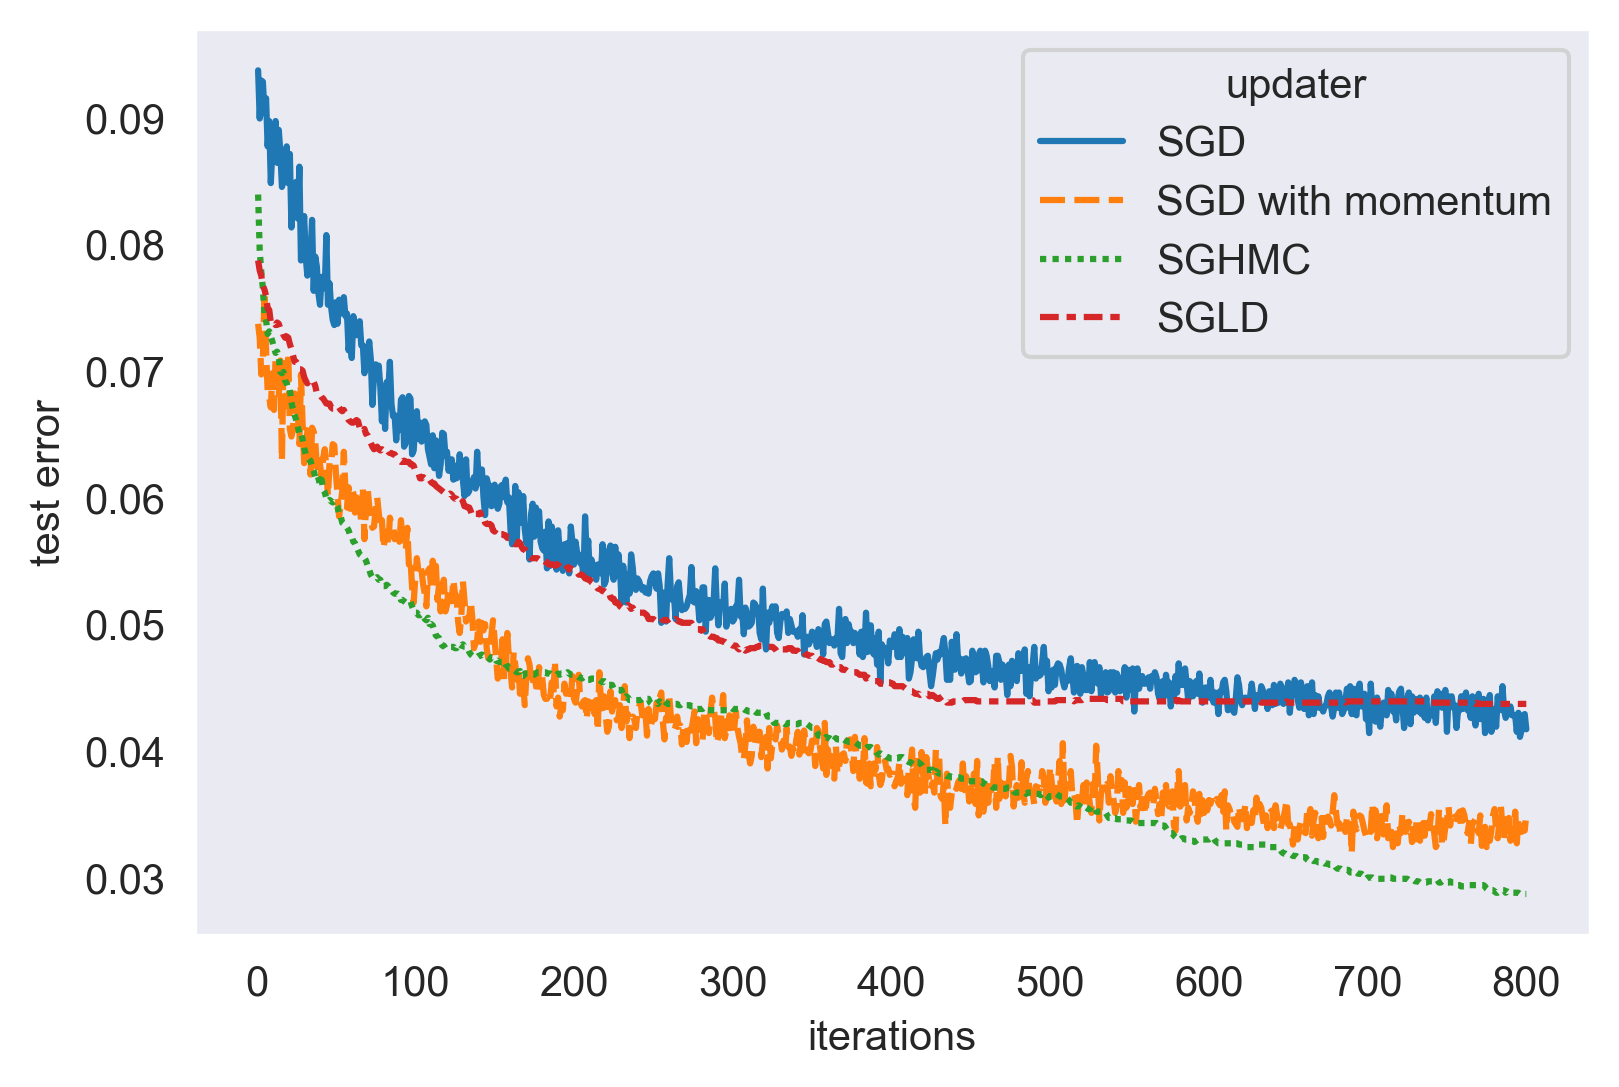
\includegraphics[width=150mm]{Images/MNIST.png}
            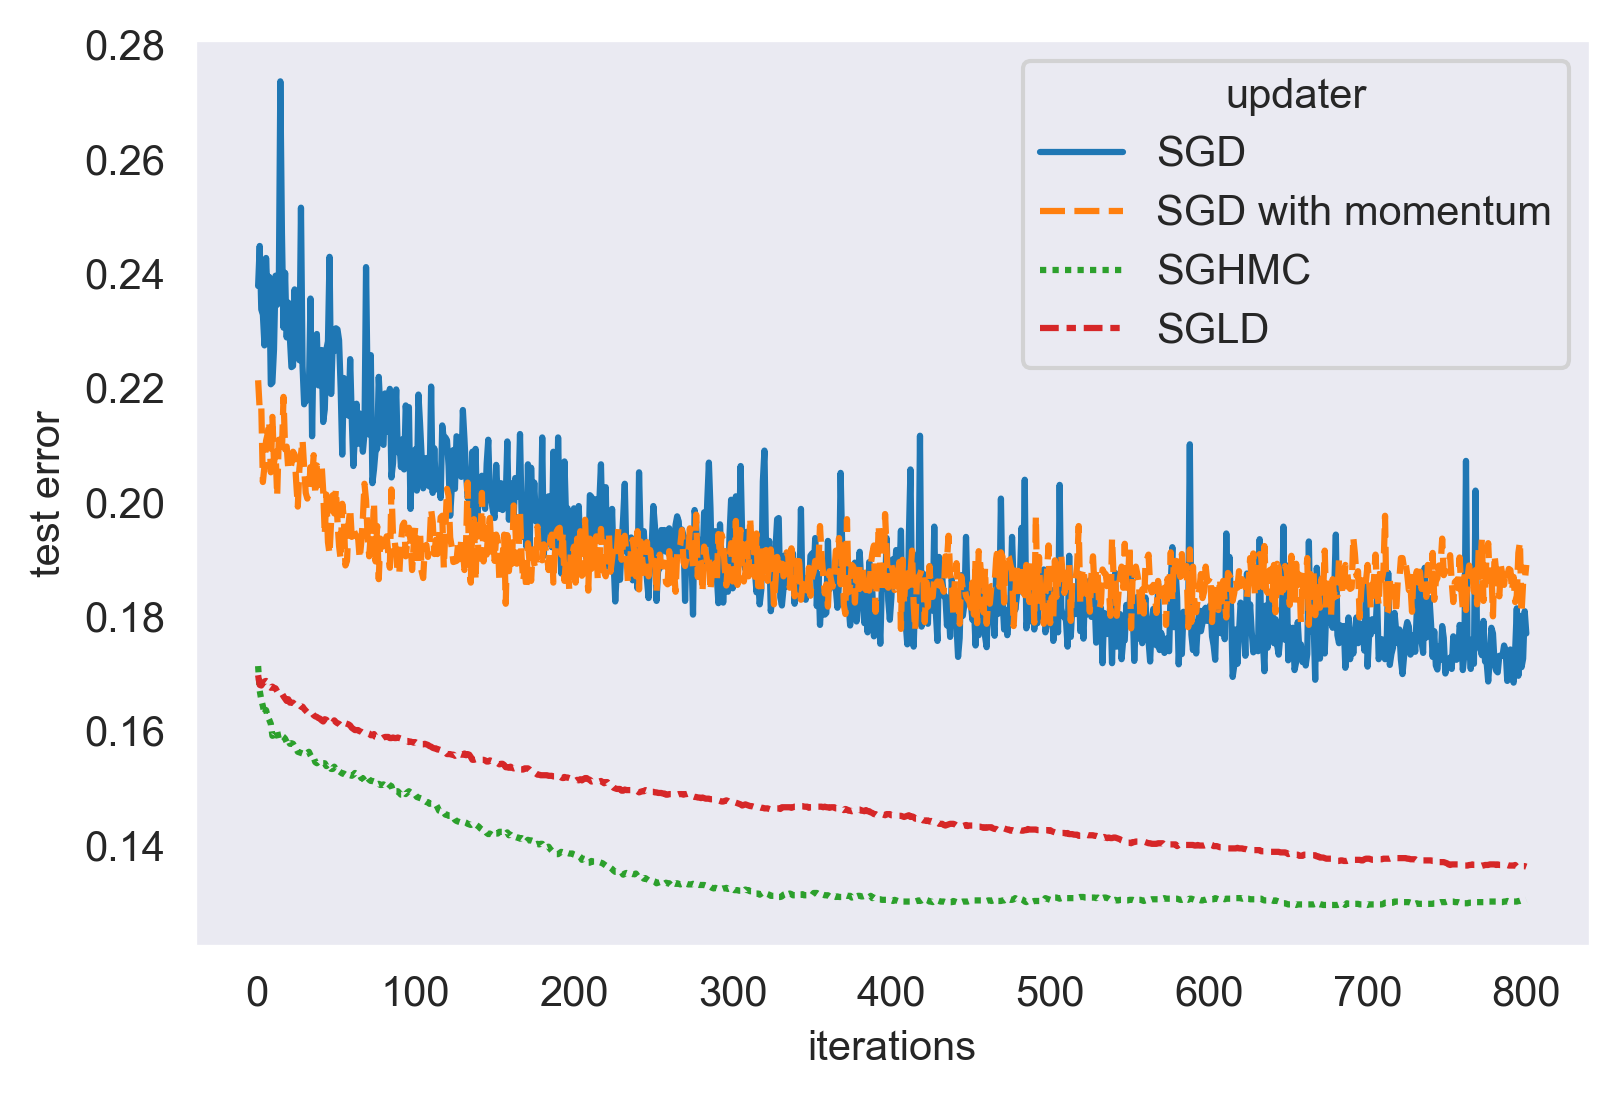
\includegraphics[width=150mm]{Images/fashion-mnist.png}
            \end{tikzfigure} 

        }
		\block{SGNUTS}{'Stochastic Gradient No U-Turn Sampler' (SGNUTS) is our novel algorithm based on the 'No U-Turn Sampler' (NUTS) produced in \cite{nuts}. NUTS removes the need for the user to pre-set the number of steps HMC performs before taking a sample. We produced SGNUTS to do the same for SGHMC. At its core, it works by repeatedly performing SGHMC steps either forward or backward in time until a 'U-turn' is seen. This is when a further step forwards in time would cause the latest sample in the trajectory to get closer to the earliest sample (or similarly for a step backwards in time). It reached accuracies of 0.94 on MNIST and 0.85 on FashionMNIST, which is similar to SGHMC (accuracies of 0.97 and 0.85 respectively). SGNUTS reaches the posterior faster than SGHMC, taking 28s to reach an accuracy of 0.87, compared to SGHMC taking 50s to reach 0.89. When at the posterior, SGNUTS takes longer than SGHMC to sample from it however.
		
		  \begin{tikzfigure}[SGNUTS Learning Curves on MNIST (left) and FashionMNIST (right)]
            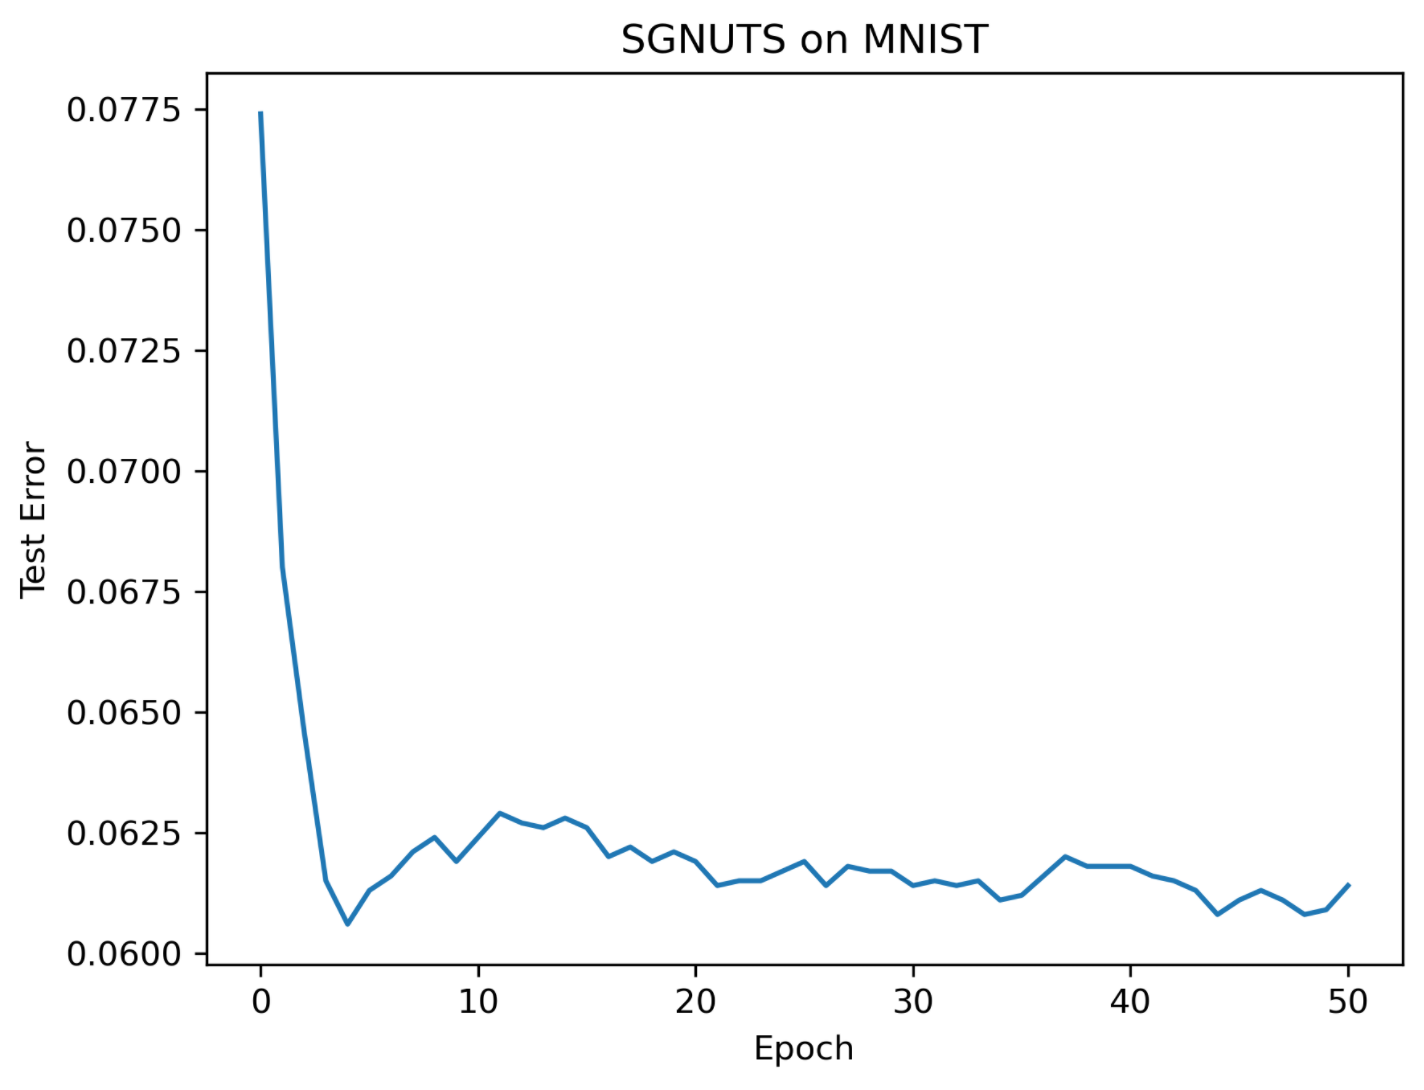
\includegraphics[width=120mm]{Images/SGNUTS_MNIST.png}
            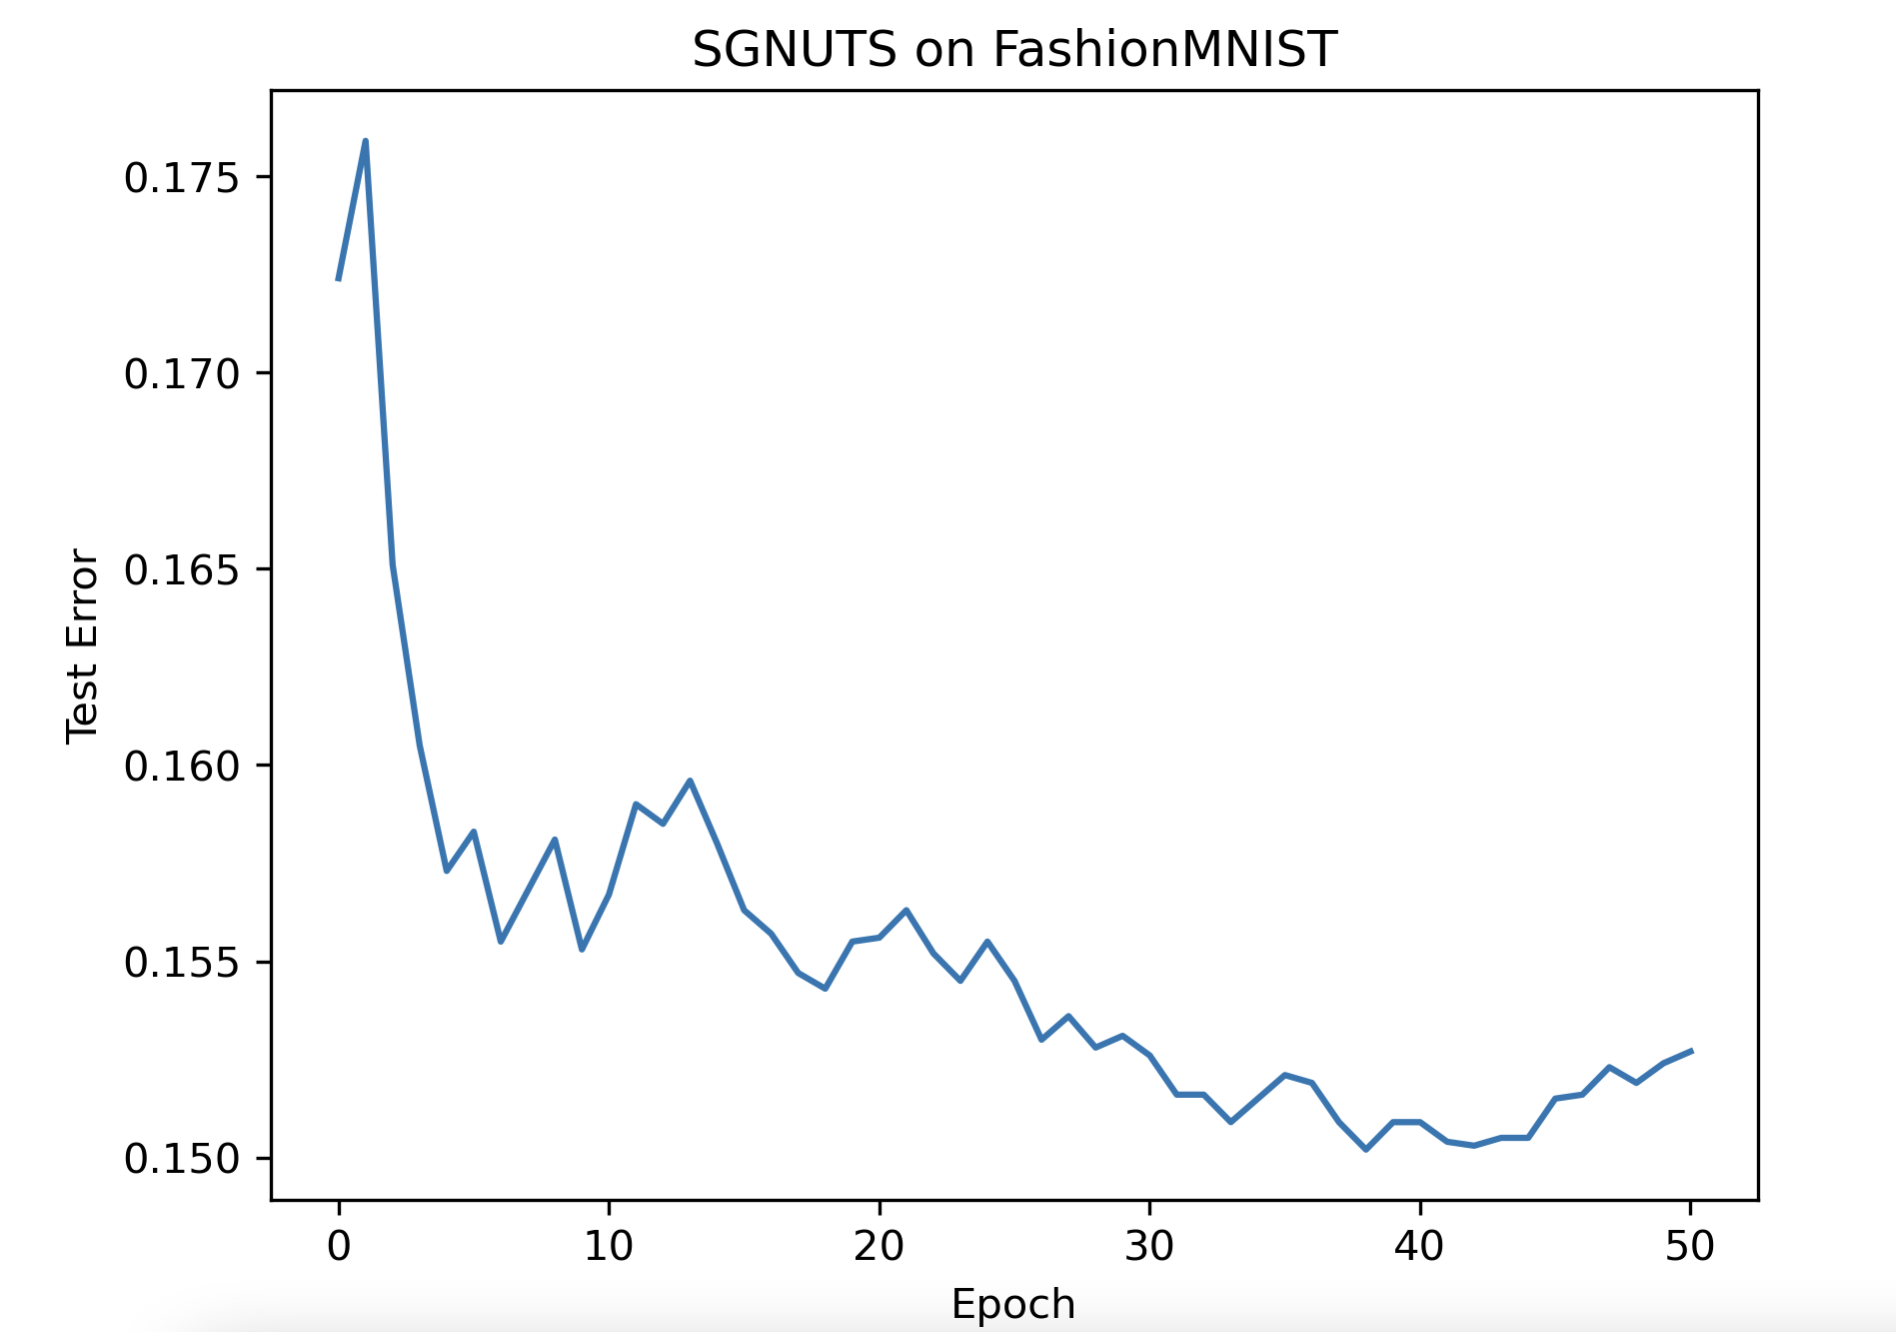
\includegraphics[width=120mm]{Images/SGNUTS_Fashion.png}
            \end{tikzfigure} }

		
		%%% Second column %%%%%%%%%%%%%%%%%%%%%%%%%%%%%%%%%%%%%%%%%%%%%%%%%%%%
		\column{0.5}
			\block{Our Reproduction and Extensions}{
	We reproduced the following experiments from the paper:
\begin{itemize}
    \item Sampling $\theta$ from the posterior with $U(\theta) = -2\theta^2 + \theta^4$ using HMC, Naive SGHMC and SGHMC
    \item Sampling $(\theta,r)$ generated from $U(\theta) = \frac{1}{2}\theta^2$ with HMC, and from $U(\theta) = \frac{1}{2}\theta^2 + \mathcal{N}(0,4)$ as a proxy for the noisy $\tilde{U}(\theta)$ in SGHMC
    \item Comparing the autocorrelation times of SGHMC and SGLD.
    \item Classifying the MNIST dataset using SGHMC as well as with SGD, SGD with momentum, and SGLD
\end{itemize} 
\begin{tikzfigure}[Figures from \cite{sghmc} which we aimed to reproduce. On left, $(\theta,r)$ samples generated from various methods. Center, $\theta$ samples generated from various methods. Right, learning curves for MNIST classification]
            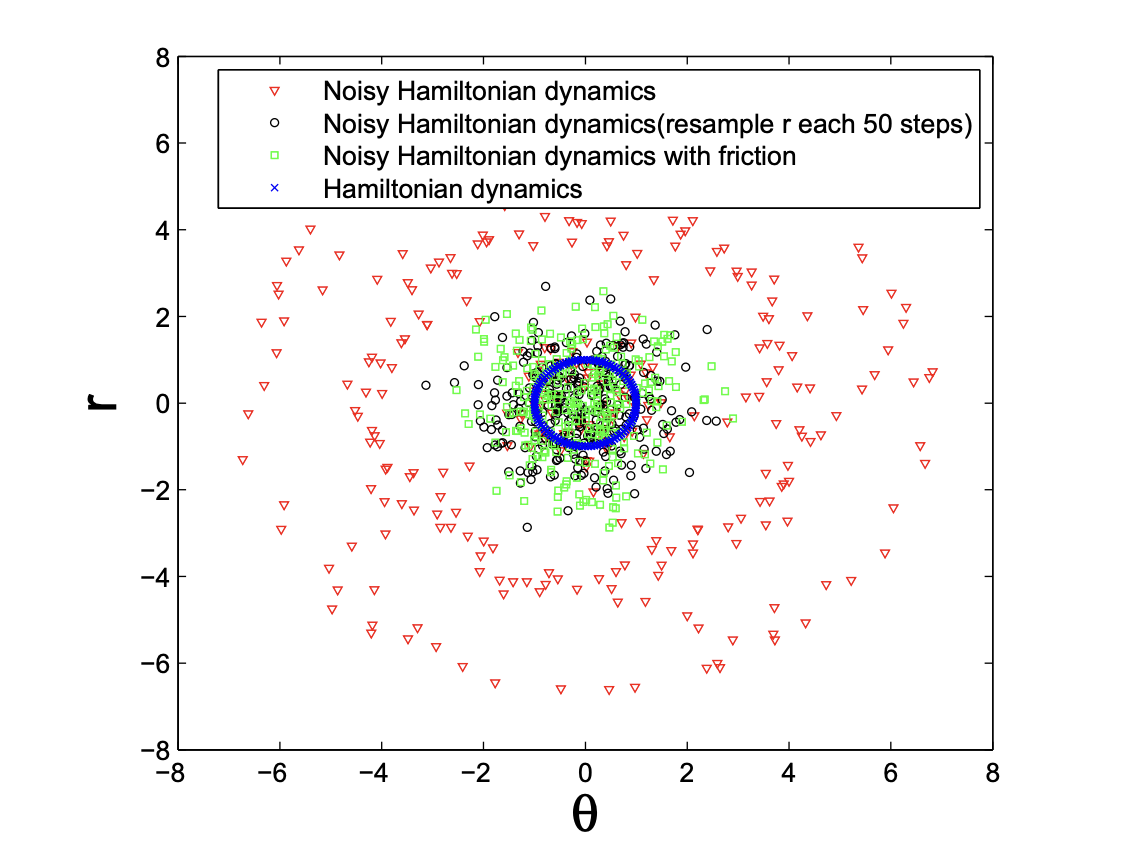
\includegraphics[width=100mm]{Images/reproduce1.png}
            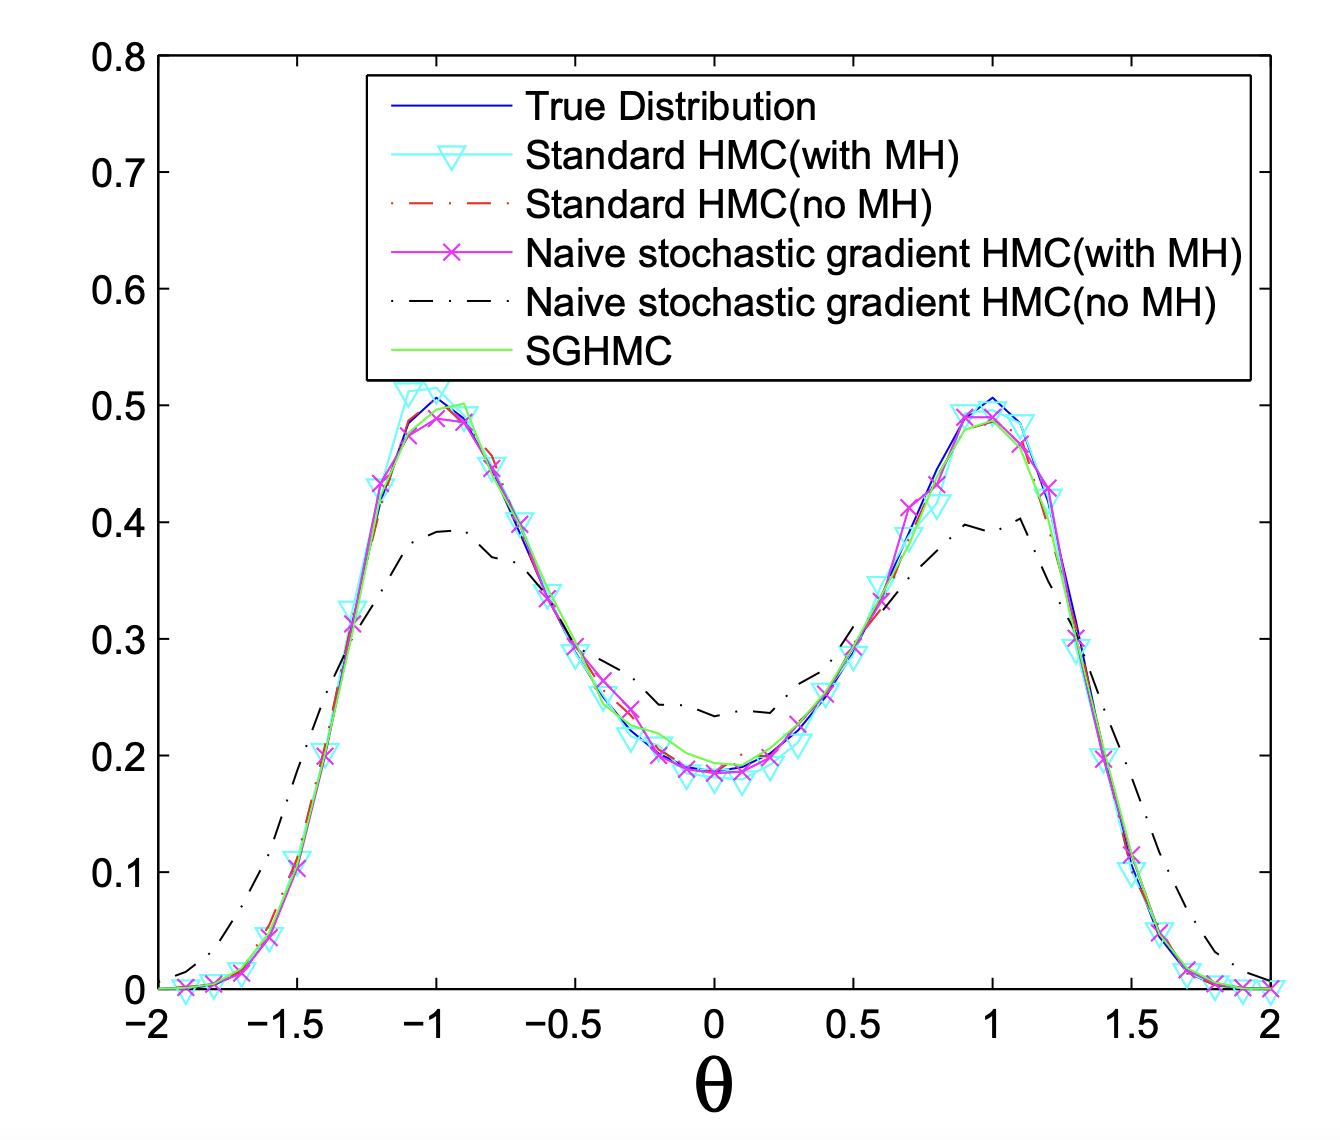
\includegraphics[width=100mm]{Images/reproduce2.png}
            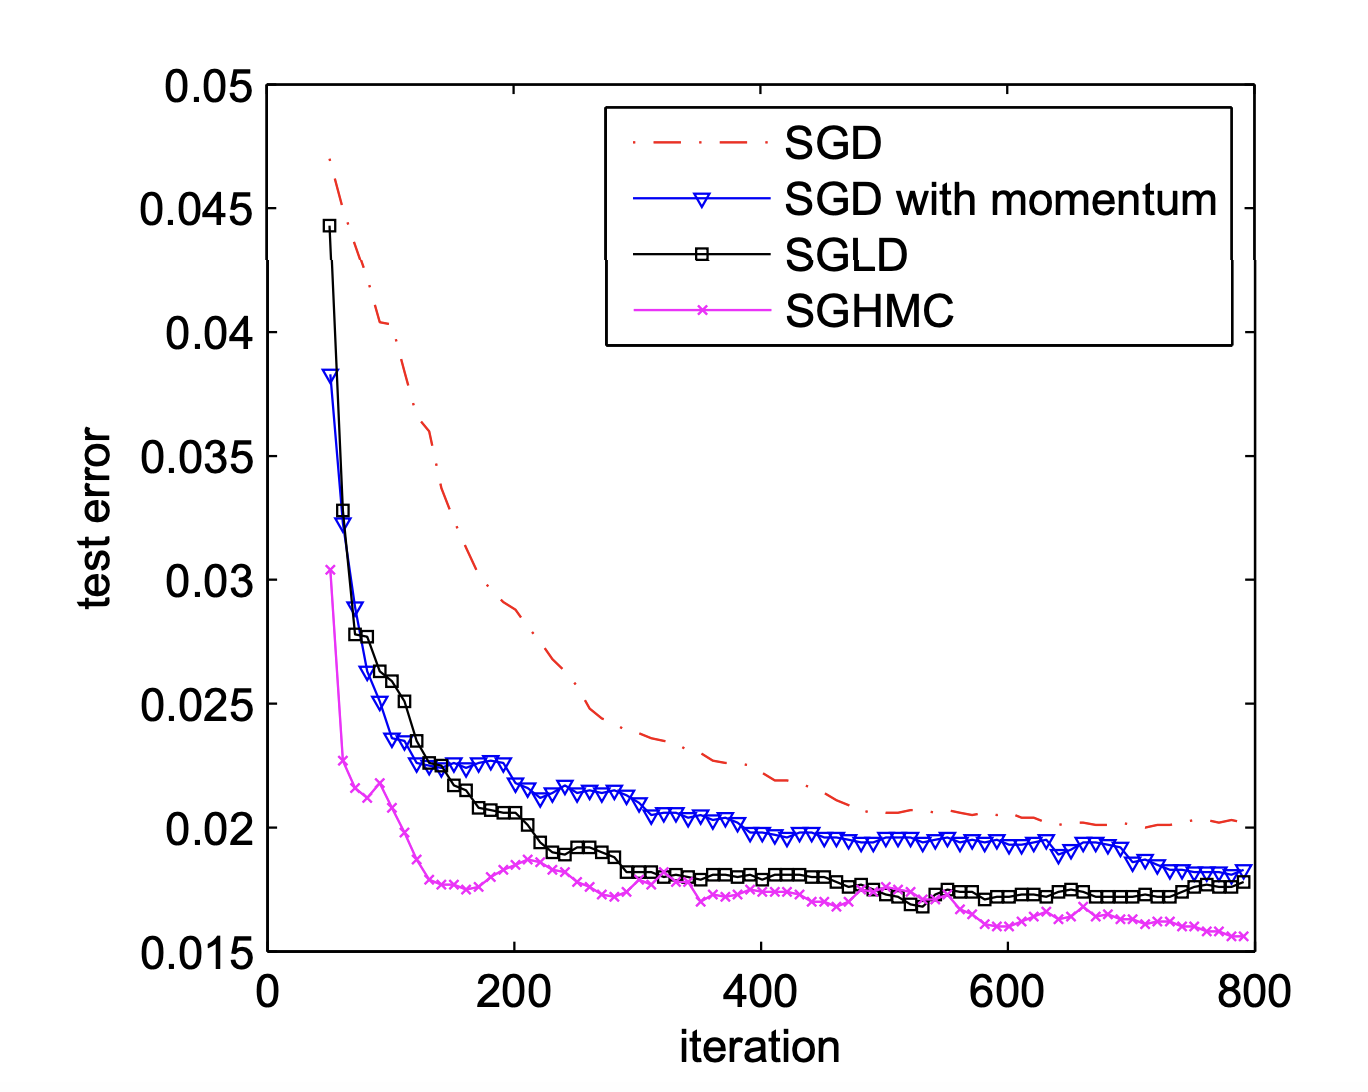
\includegraphics[width=100mm]{Images/reproduce3.png}
            \end{tikzfigure}

		We extended the results of \cite{sghmc} in the following ways:
		
	\begin{itemize}
    \item We extended the 'No U-Turn Sampler' (NUTS) from \cite{nuts} to work with SGHMC to produce our novel algorithm SGNUTS
    \item We ran experiments on a new dataset of FashionMNIST
    \item We briefly introduced some Convolutional Neural Networks (CNNs) to see how accurate SGHMC was at classifying CIFAR10
    \item We attempted to evaluate the noisiness of the data ($B$ in the literature and in what follows) and used this to increase the algorithm's efficiency
\end{itemize}
		
	}

    		\block{Implementation Details}{We implemented the following algorithms from scratch: HMC, SGHMC, SGLD , SGD, SGD with Nesterov momentum and SGNUTS. All of our implementations subclass Pyro's \texttt{MCMCKernel} and are designed to be used directly with Pyro \cite{pyro} — a universal probabilistic programming language (PPL) written in Python. Pyro comes with useful built in functions that transform probabilistic programs (PP) into potential functions that automatically handle gradient computations. The main caveat of stochastic gradient samplers and optimizers is that we require that the potential function has the form: $$\widetilde{U}(\theta) =  -\frac{|D|}{|\widetilde{D}|} \log p(\widetilde{D} \: | \: \theta) - \log p (\theta)$$
Using our implementations we illustrate below how sampling algorithms differ from optimization algorithms; while sampling algorithms visit the full posterior $p(\theta \: | \: D)$ as they draw samples, optimization algoithms hone in on the MAP estimate $\text{argmax}_{\theta} \{ p(D \: | \: \theta) \cdot p(\theta) \}$. 
	\begin{tikzfigure}[{\bf Far left}: SGHMC (\texttt{batch\_size} $= 5, \eta = 0.01, \alpha=0.1$ \texttt{num\_steps}$=10$, \texttt{resample\_n} $=50$). {\bf Mid left:} SGLD (\texttt{batch\_size} $= 5, \eta = 0.1, \alpha=0.1$ \texttt{num\_steps}$=5$). {\bf Mid right:} SGD (\texttt{batch\_size} $= 5, \eta = 0.001$). {\bf Far right:} SGD with Nesterov momentum (\texttt{batch\_size} $= 5, \eta = 0.001, \alpha=0.1$)]
            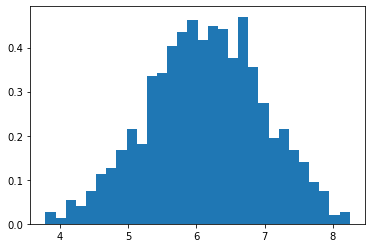
\includegraphics[width=75mm]{Images/SGHMC_demo.png}
            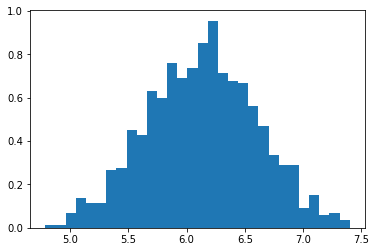
\includegraphics[width=75mm]{Images/SGLD_demo.png}
	    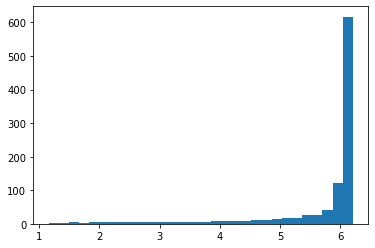
\includegraphics[width=75mm]{Images/SGD_demo.png}
            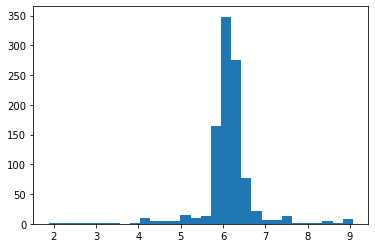
\includegraphics[width=75mm]{Images/SGDMOM_demo.png}
            \end{tikzfigure}
 }
		
\block{Simulated Examples}{
			Simulated scenarios are reproduced and extended from scratch based on the Matlab version of the original paper \cite{simu_code}. Conclusions can be drawn as follows:
		\begin{itemize}
        \item As shown in Fig. 5(a), compared with naive stochastic gradient HMC, which requires a frequent costly MH correction step, SGHMC maintains more perfectly on both of the desired target distributions.
        \item As shown in Fig. 5(b), compared with naive stochastic gradient HMC without MH, which may not yield the correct target distribution, SGHMC can be used to modify the noisy dynamical system more correctly. The extension on the step size in Fig. 2(b) proves the Theorem 3.1 that $p_t(\theta,r)$ tends to be a uniform distribution over time, which can be very far from the target distribution $\pi$.
        \item As shown in Fig. 5(c), as step size decreases, SGLD \cite{sgld} has a high autocorrelation time while SGHMC has very low one with even lower estimation error which indicates the efficiency of SGHMC. Fig. 5(d) shows that SGLD performs worse to explore the tails of the distribution compared to SGHMC.
        \end{itemize} 
	\begin{tikzfigure}[{\bf (a)}: Points $(\theta,r)$ simulated of 15000 steps. {\bf (b):} Points $(\theta,r)$ simulated of 150000 steps. {\bf (c):} Autocorrelation time versus estimation error for the five settings. {\bf (d):} First 50 samples of SGHMC and SGLD]
	   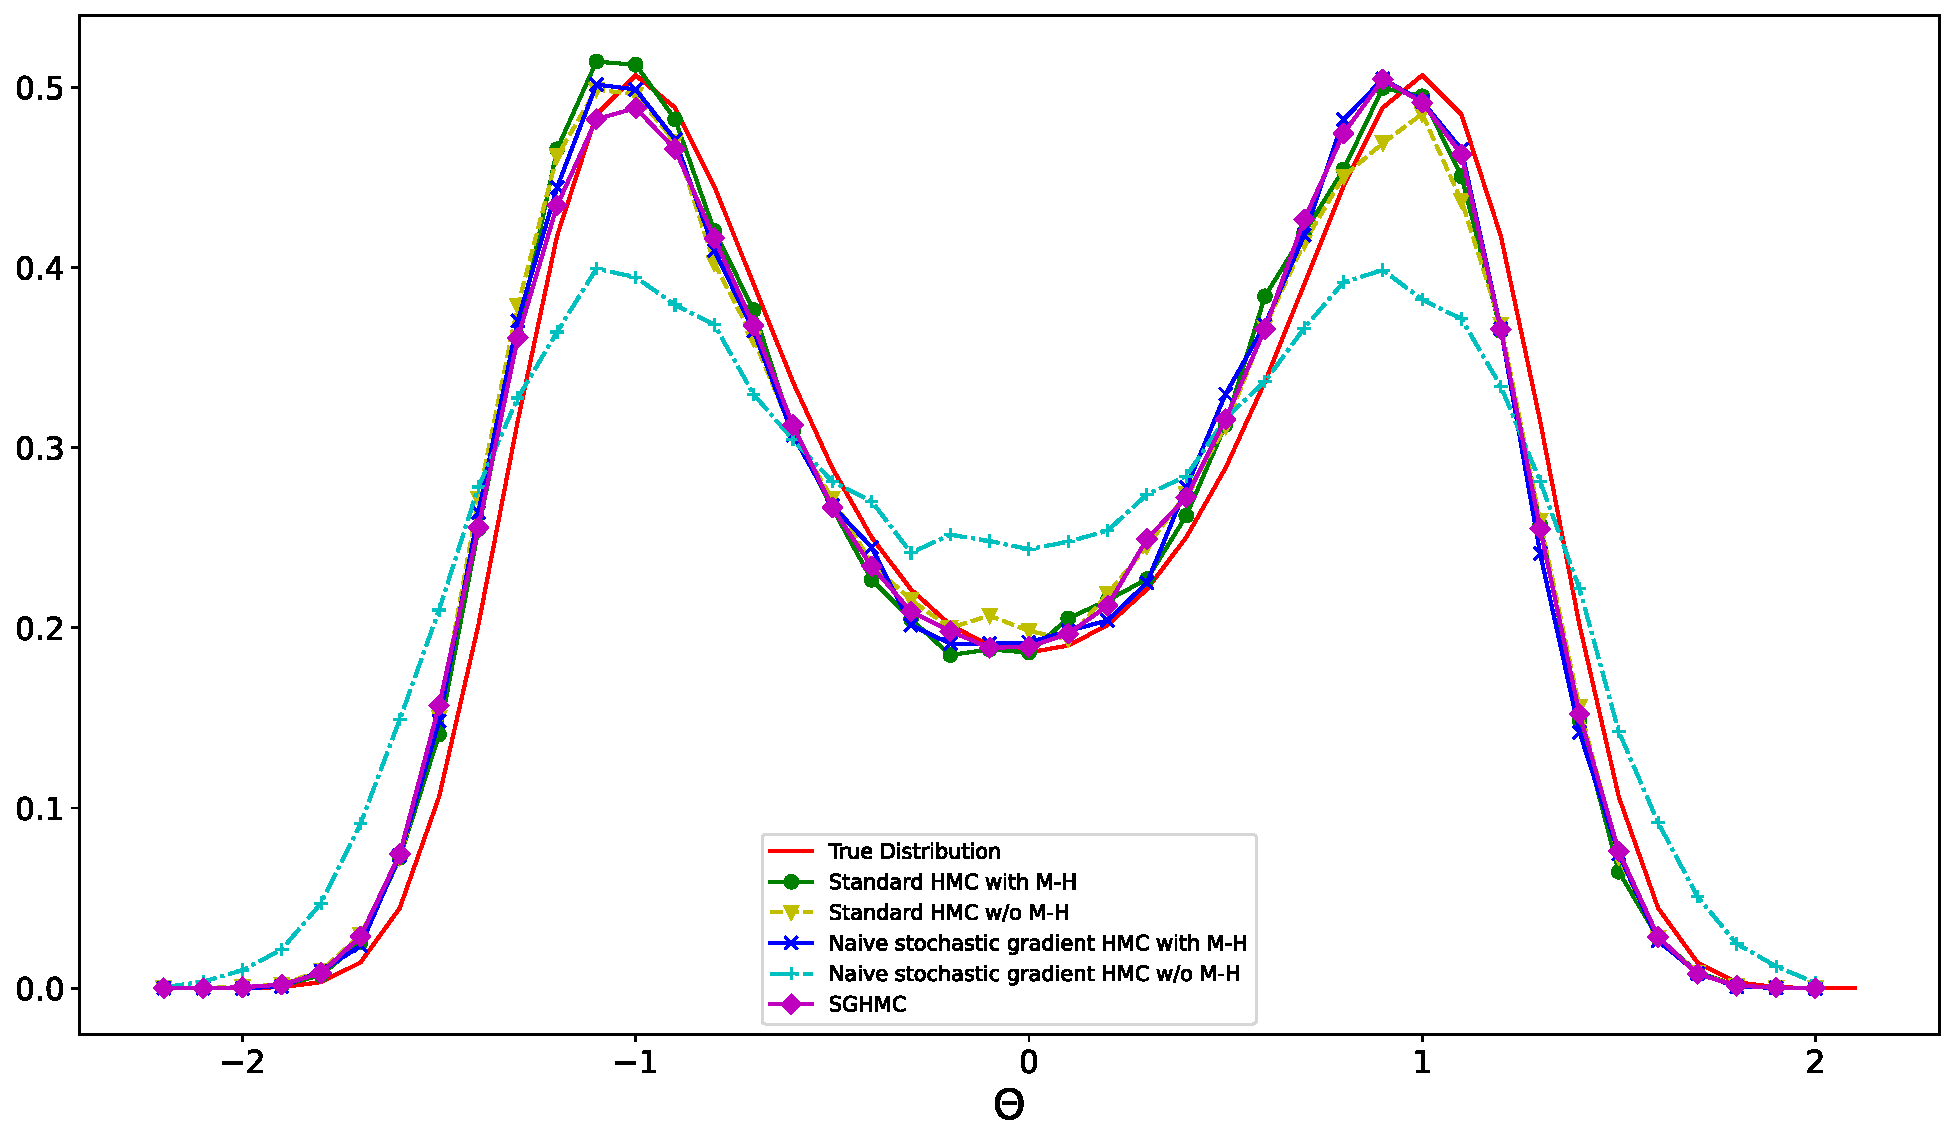
\includegraphics[width=120mm]{Images/fig1ax4.pdf}
            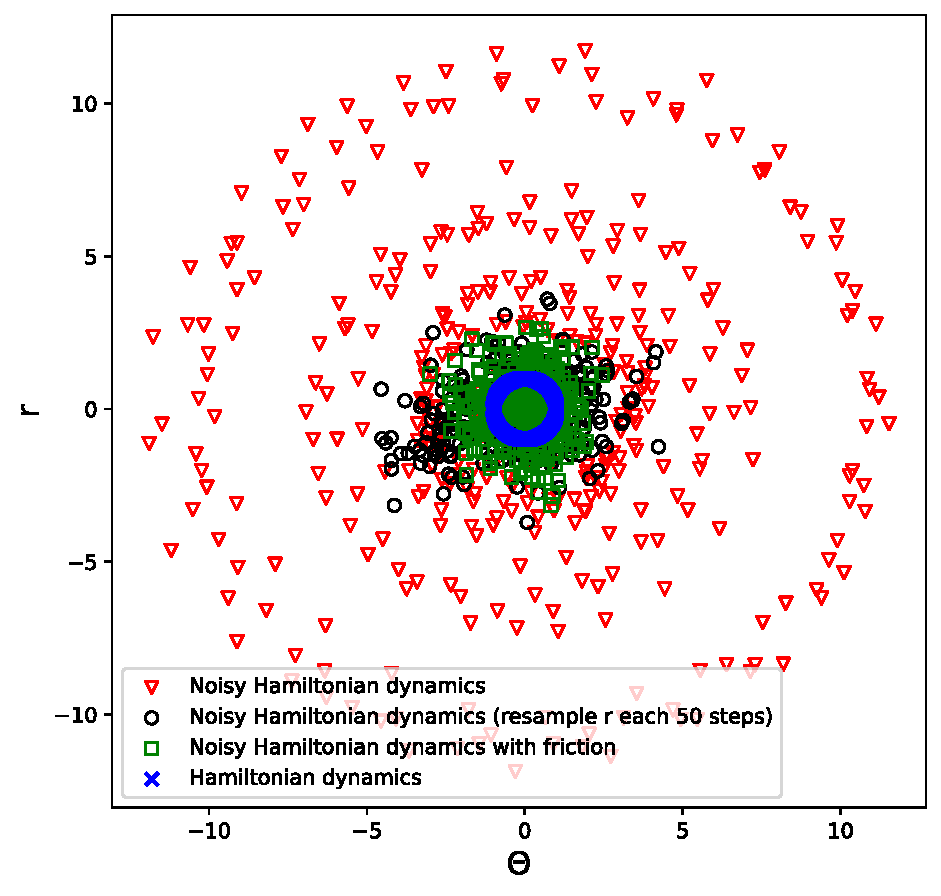
\includegraphics[width=75mm]{Images/fig2apt.pdf}
	    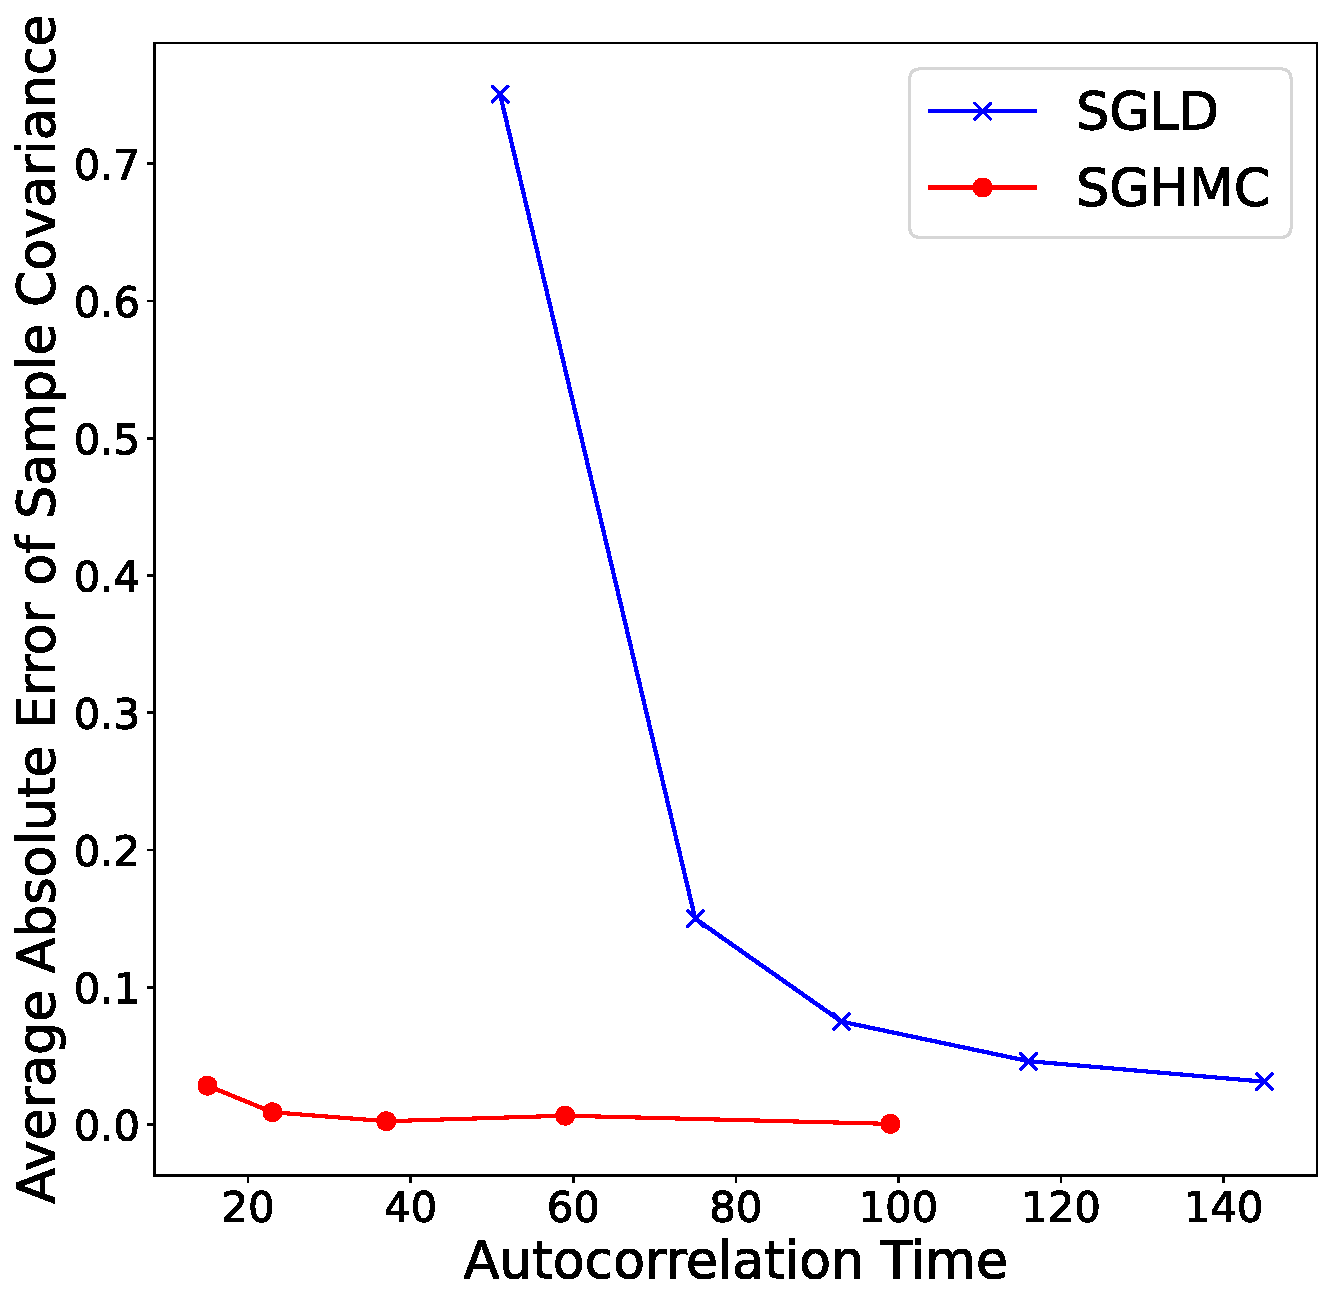
\includegraphics[width=75mm]{Images/fig3aerrt.pdf}
            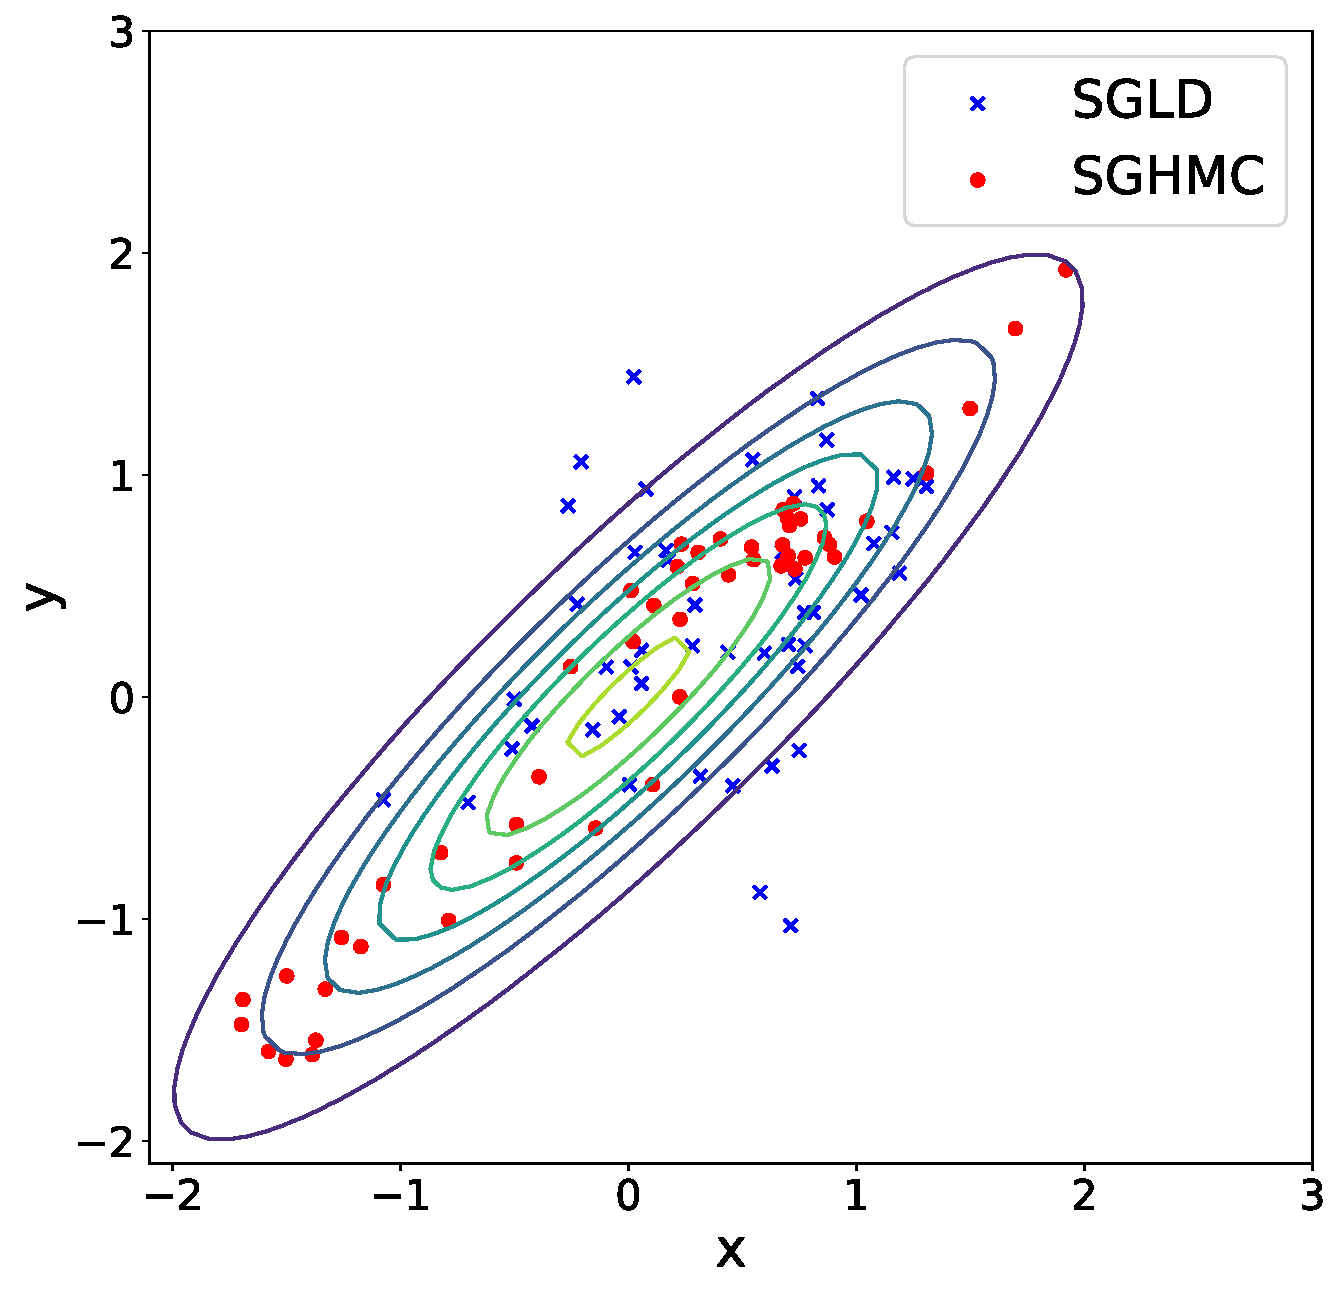
\includegraphics[width=75mm]{Images/fig3btraj.pdf}
            \end{tikzfigure} 		
	}
		
		\block{Further Research}{
		\begin{itemize}
		    \item Implementation of a joint SGNUTS and SGHMC algorithm - SGNUTS quickly reaches the posterior, however SGHMC is faster at sampling when at the posterior. We could investigate the power of using SGNUTS for the first few epochs, followed by SGHMC.
		   \item Fine-tuning the CNN used to classify CIFAR10. Currently we have shown that our SGHMC implementation can start classifying CIFAR10, however our accuracies could be higher with more time to fine-tune it.
		   \item Investigate further methods of estimating the noise model $B$, as using empirical Fisher was computationally expensive
		   \item Compare thoroughly with the more popularly used Variational Inference Method.
		\end{itemize}		}
		

	
	\end{columns}
	
			\block{References}{
		\printbibliography[heading=none]
}


\end{document}